\section{Controller in time domain}

% State feedback controller
\subsection{State feedback controller}
In a first time, one needs to compute the gain matrix $K$.\par
In order not to apply a gain on the wind force, the matrix K is as follows :
$$
K = \begin{pmatrix}
    0 & 0 & 0 & 0\\ 
    g_1 & g_2 & g_3 & g_4
\end{pmatrix}
$$
Indeed, the first column of matrix B concerns the uncontrollable input, so matrix K cannot affect these values.\par
The new dynamic matrix of the closed-loop system is $A_{CL} = A - BK$. Let's determine the eigenvalues of that matrix.\par
As one has a matrix of dimension $4$, the approximation of the dominant poles will be done. Indeed, one has, from the previous matrix $A$, the eigenvalues :
\begin{align*}
    \lambda_1 &= \num{-0.0634 + 6.2837i}\\
    \lambda_2 &= \num{-0.0634 - 6.2837i}\\
    \lambda_3 &= \num{-0.1666 + 1.8179i}\\
    \lambda_4 &= \num{-0.1666 - 1.8179i}
\end{align*}
As already discussed in section \ref{sec:eigenvalues}, one can see that $\lambda_3$ and $\lambda_4$ are about 10 times bigger than the last two, and so they do not require any modification. Those two will therefore remain in $A_{CL}$.\par
Imposing that $(s - \lambda_3)(s - \lambda_4)$ is part of the decomposition, one gets that the determinant of $A_{CL}$ is equal to :
$$
(s - \lambda_3)(s - \lambda_4)(s^2 + 2 \xi\omega_c s + \omega_c^2) = 0
$$
Since $\lambda_3$ and $\lambda_4$ are fixed, one only needs to solve the equation of the second degree in $s$ in order to find the expressions of $\lambda_1'$ and $\lambda_2'$ as a function of $\xi$ and $\omega_c$.\par
The solutions of the equation are given by :
$$
\begin{cases}
    \lambda_1' = -\xi\omega_c - \omega_c\sqrt{\xi^2 - 1}\\
    \lambda_2' = -\xi\omega_c + \omega_c\sqrt{\xi^2 - 1}
\end{cases}
$$
The values of $\xi$ and $\omega_c$ will be determined by simulations in the following sections. When these have been fixed, the values of the 4 poles of $A_{CL}$ will be obtained. Then one will just have to use the \texttt{place} function of Matlab to obtain the values $g_i$ of matrix $K$ associated with the eigenvalues.\par
However, as previously noted via simulations, our system is very reactive. The two eigenvalues have x and y have also been modified to slow down the system. We finally obtain the expressions of the 4 eigenvalues of the controller :
$$
\begin{cases}
    \lambda_1' = -\xi\omega_c - \omega_c\sqrt{\xi^2 - 1}\\
    \lambda_2' = -\xi\omega_c + \omega_c\sqrt{\xi^2 - 1}\\
    \lambda_3' = \mathbb{R}(\lambda_3)0.5 + \mathbb{I}(\lambda_3)i\\
    \lambda_4' = \mathbb{R}(\lambda_4)0.5 + \mathbb{I}(\lambda_3)i
\end{cases}
$$
As the reference is 0, $k_r$ has not to be considered, so it can fixed to 0.\par
However, if the reference was to change, one could compute $k_r$, it would be nice. Some tests of a change in reference will be performed in this report. We therefore calculated $k_r$ using the following formula :
$$
k_r = \frac{-1}{C(A - BK)^-1 B}
$$
where only the controllable part of matrix B (second column) was considered. Indeed, if the entire matrix were used, it would mean that we would have an action on the uncontrollable input, which is not possible.

% Observer
\subsection{Observer}
The controllable input being a linear combination of the different states multiplied by gains, the control system requires the different states as inputs. However, the open loop system only provides one output.\par
Considering that the real states cannot be measured in practice, the observer is a tool that allows, based on the output of the open loop system only, to approximate the different states of the system to control it.\par
Its realization must be such that the convergence of the estimated states with the real states is as fast and correct as possible.
One thus needs to compute the gain matrix $L$ :
$$
L = \begin{pmatrix}
    l_1\\
    l_2\\
    l_3\\
    l_4
\end{pmatrix}
$$
The new dynamic matrix is given by $A_{obs} = A - LC$.\par
As previously, one will keep the same two dominant eigenvalues and determine the two other via the same method that has been used for $K$.\par
Imposing that $(s - \lambda_3')(s - \lambda_4')$ is part of the decomposition, one gets that the determinant of $A_{obs}$ is equal to :
$$
(s - \lambda_3')(s - \lambda_4')(s^2 + 2 \xi\omega_c s + \omega_c^2) = 0
$$
Since $\lambda_3'$ and $\lambda_4'$ are fixed, one only needs to solve the equation of the second degree in $s$ in order to find the expressions of $\lambda_1*$ and $\lambda_2*$ as a function of $\xi$ and $\omega_c$.\par
The solutions of the equation are given by :
$$
\begin{cases}
    \lambda_1* = -\xi\omega_c - \omega_c\sqrt{\xi^2 - 1}\\
    \lambda_2* = -\xi\omega_c + \omega_c\sqrt{\xi^2 - 1}
\end{cases}
$$
The poles of the observer are determined by taking the poles of the controller and moving them. To do this, the real parts of each pole are multiplied by a constant $\alpha$. In the case of poles $\lambda_1'$ and $\lambda_2'$, this amounts to multiplying $\omega_c$ by $\alpha$.\par
One finally has :
$$
\begin{cases}
    \lambda_1* = -\xi\omega_c\alpha - \omega_c\alpha\sqrt{\xi^2 - 1}\\
    \lambda_2* = -\xi\omega_c\alpha + \omega_c\alpha\sqrt{\xi^2 - 1}\\
    \lambda_3* = \mathbb{R}(\lambda_3')\alpha + \mathbb{I}(\lambda_3')i\\
    \lambda_4* = \mathbb{R}(\lambda_4')\alpha + \mathbb{I}(\lambda_4')i
\end{cases}
$$
The values $l_i$ of the matrix $L$ are then obtained by using the \texttt{place} function of Matlab.

% Simulations and discussion
\subsection{Simulations and discussion}
\subsubsection{Parameter determination}
In order to best achieve our control system, we must determine the values of $\xi$, and $\omega_c$. We know that the system control is done via the controllable input $u(t)$, and that this input will influence the variation of the output and the different states of the system.\par
In order to obtain a coherent system, {\it i.e.} physically possible state values and an attenuation of building oscillations, we must choose values of $\xi$ and $\omega_c$ that will lead to a control input making the system coherent.\par
We tested several values of $\xi$ as well as several values of $\omega_c$ with a constant wind force :
\begin{figure}[H]
    \centering
    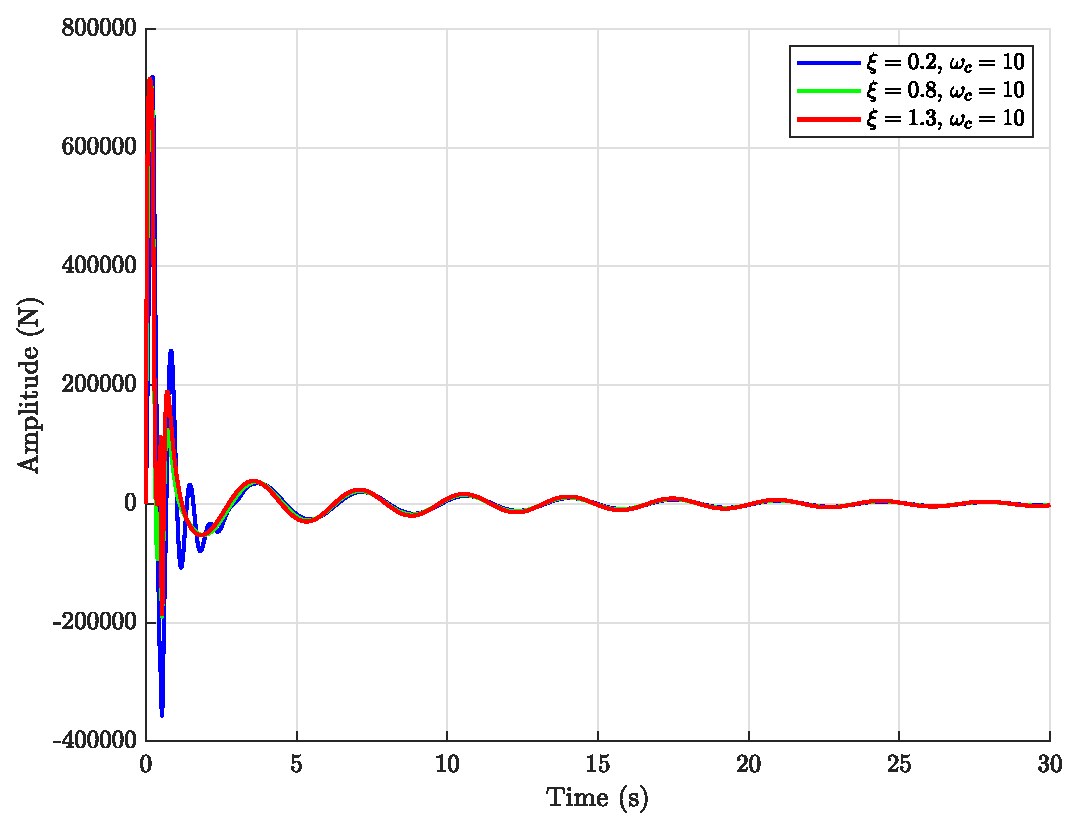
\includegraphics[width=\textwidth]{resources/eps/xi-variations.eps}
    \caption{Control input $u(t)$ for different variations of parameter $\xi$}
\end{figure}
\begin{figure}[H]
    \centering
    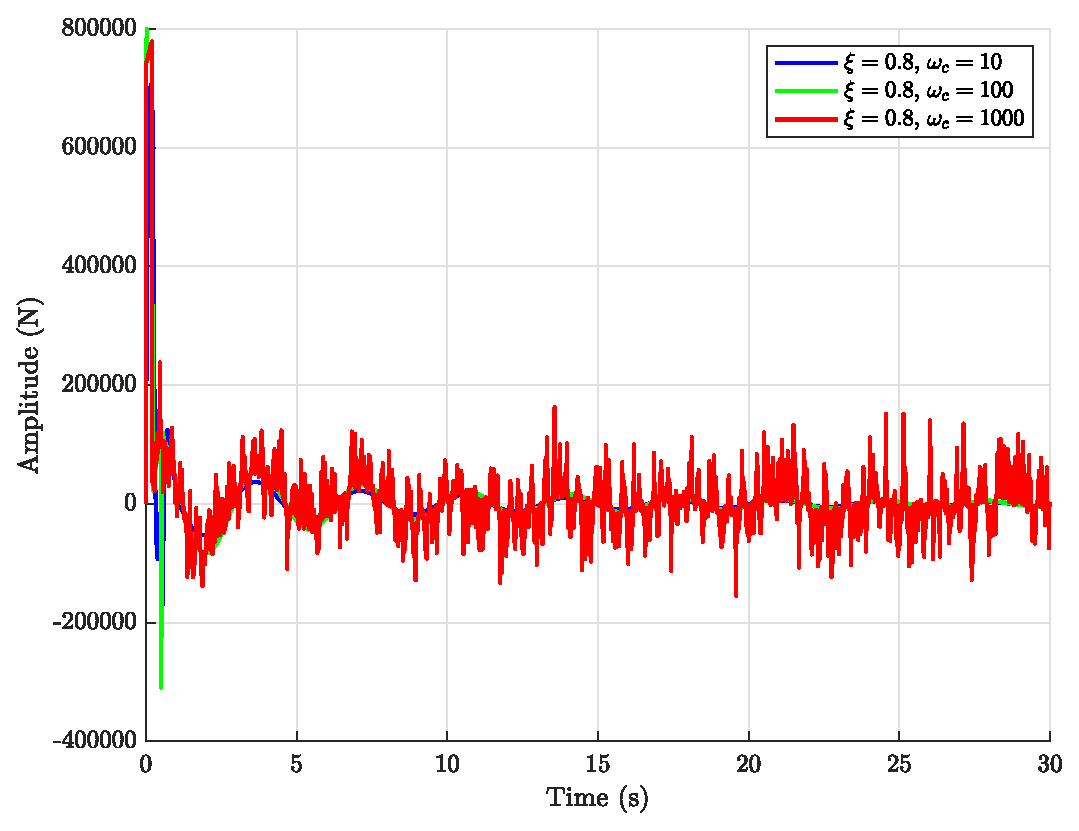
\includegraphics[width=\textwidth]{resources/eps/omega-variations.eps}
    \caption{Control input $u(t)$ for different variations of parameter $\omega_c$}
\end{figure}
It can be seen that the variations in parameter $\xi$ have little influence on the controllable force : after a few seconds, it is identical in all cases.\par
Concerning the parameter $\omega_c$, we observe that the higher it is, the faster the control force oscillates (which is an undesirable behaviour).\par
We therefore choose to take the following values of the parameters :
$$
\begin{cases}
    \xi = \num{0.8}\\
    \omega_c = \num{10}
\end{cases}
$$
We also arbitrarily choose our parameter $\alpha = 5$. This choice, in view of the simulations presented later, is proving to be a good one.\par
With these different values, our control input is as follows :
\begin{figure}[H]
    \centering
    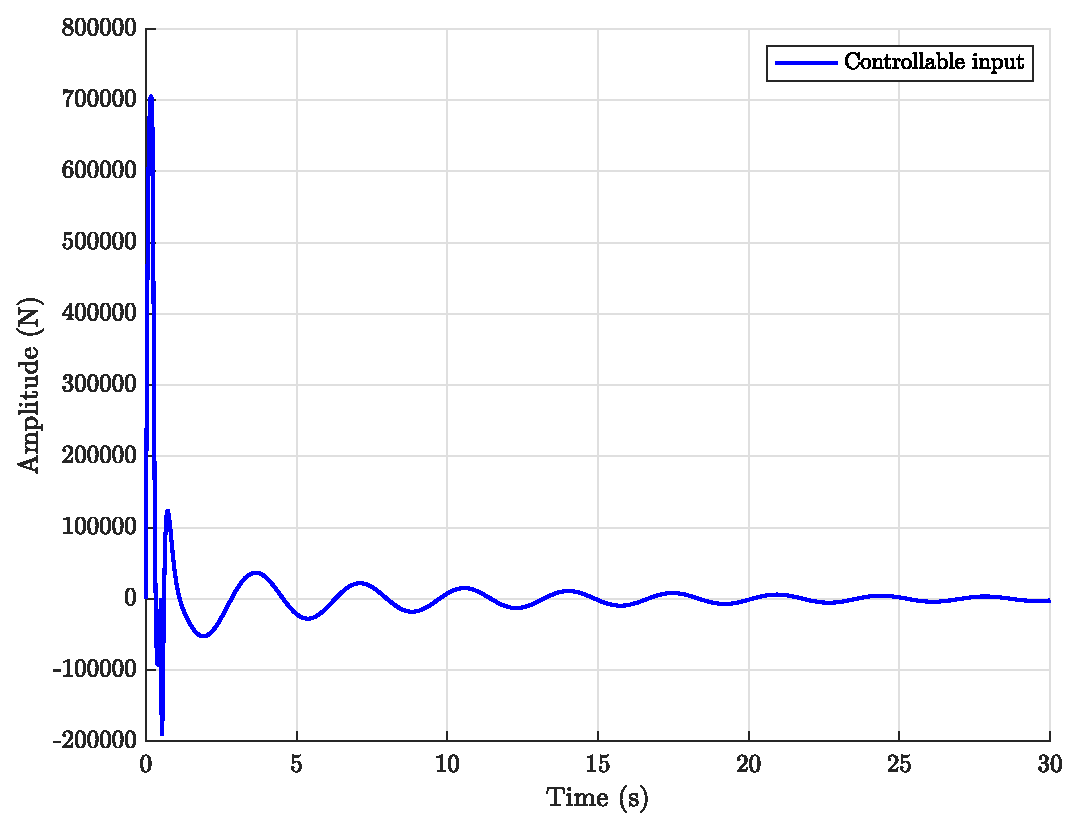
\includegraphics[width=\textwidth]{resources/eps/controllable-input.eps}
    \caption{Control input $u(t)$ for $\xi = \num{0.8}$ and $\omega_c = \num{10}$}
\end{figure}
An abnormally high peak is observed at the beginning. This peak is due to the unrealistic simulations performed : the simulation goes from a zero wind to a constant wind of several thousand newtons in an instant (similar to a step). However, it can be seen that after this peak, the control force oscillates around much more realistic values within our previously defined acceptable range of values.\par
This control input does allow a reduction in building oscillations, and this in a relatively slower way (the system has been slowed down).
\begin{figure}[H]
    \centering
    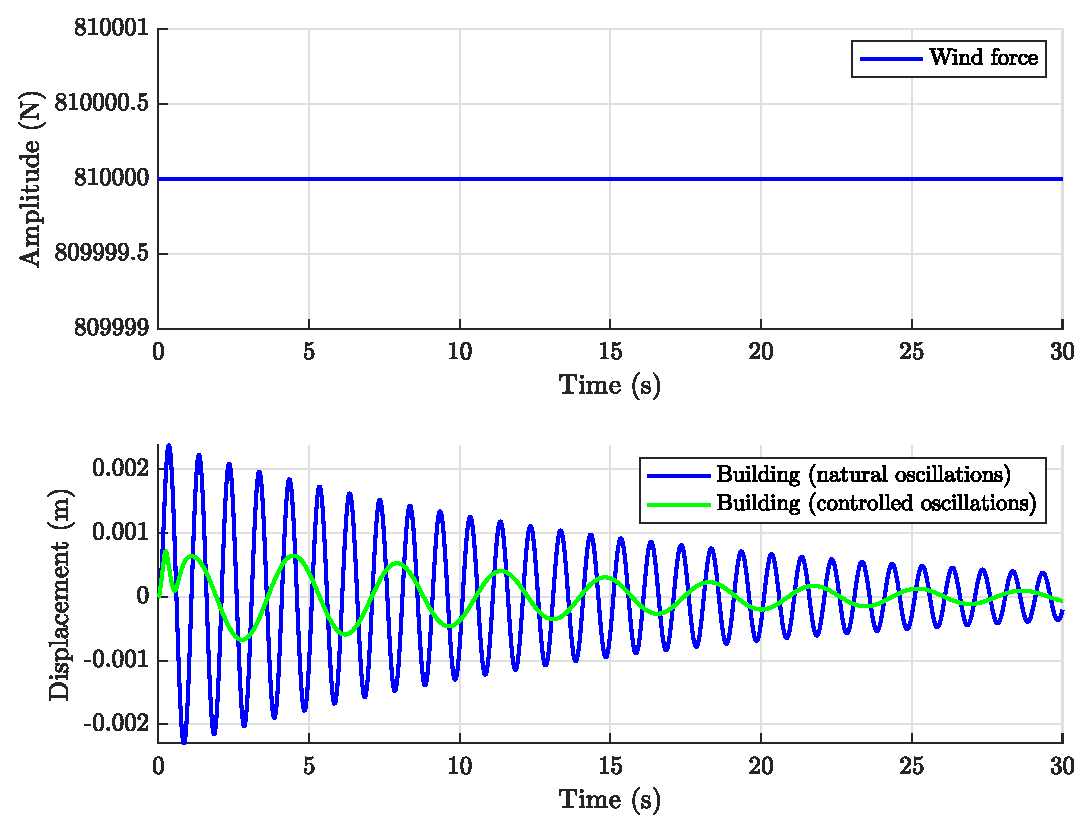
\includegraphics[width=\textwidth]{resources/eps/controller.eps}
    \caption{System simulation with and without control input}
\end{figure}
We will now study the behaviour of the system in several situations. In order to judge its quality, the results of the observation will be displayed. The output of the system being also its first state, it can be studied by observing the first state to observe it.

\subsubsection{Response to a reference variation}
For this simulation, we have set the uncontrollable input to 0 and changed the reference to \SI{0.002}{\meter}.
\begin{figure}[H]
    \centering
    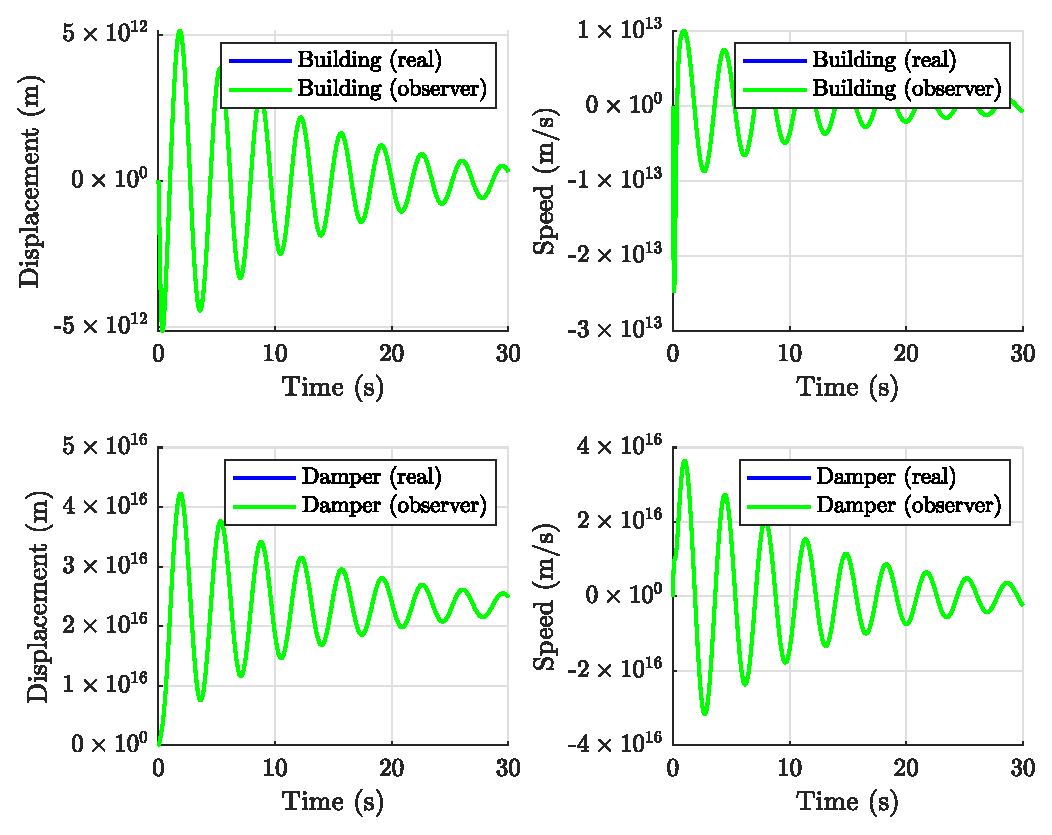
\includegraphics[width=\textwidth]{resources/eps/observer-reference.eps}
    \caption{System and observer simulation with a reference variation of \SI{0.002}{\meter}}
\end{figure}
comments to do

\subsubsection{Response to a perturbation (disturbance)}
In order to study the convergence of the observer towards real states, we added a delay to the entry of the observer.\par
We simulated our different wind scenarios to see how the controlled system reacts and to check if the convergence of the observer is good.
\begin{figure}[H]
    \centering
    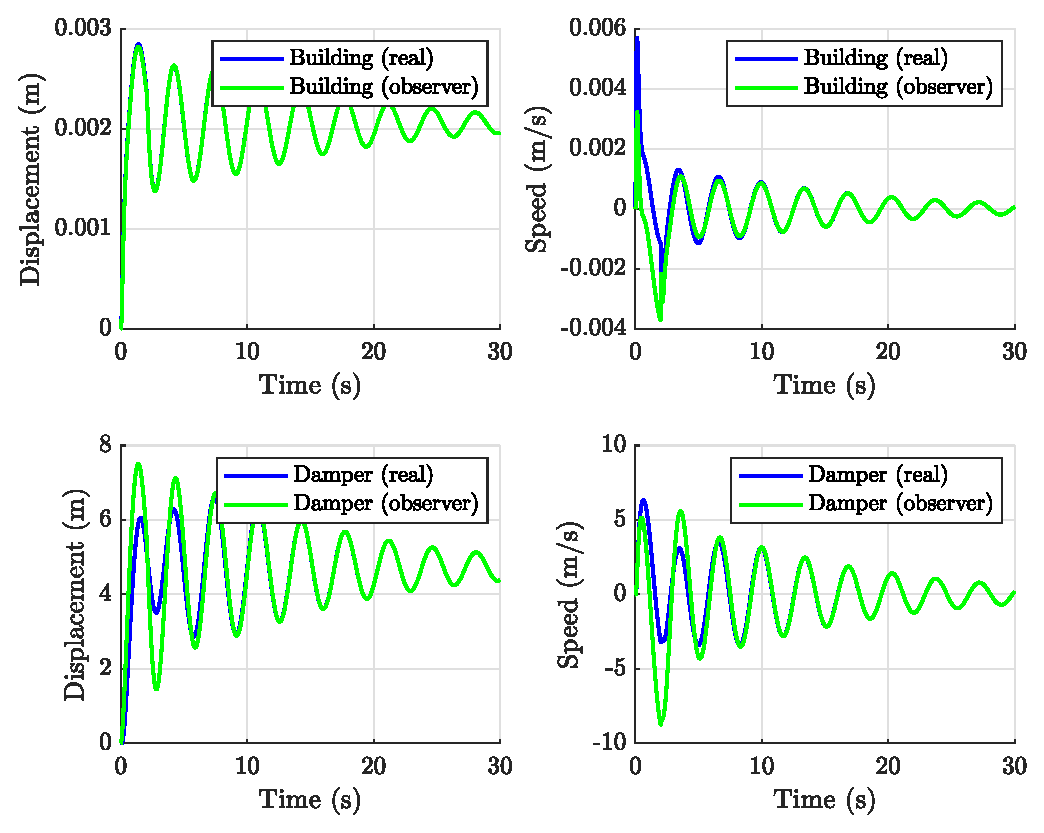
\includegraphics[width=\textwidth]{resources/eps/observer-constant.eps}
    \caption{System and observer simulation with a constant wind force}
\end{figure}
\begin{figure}[H]
    \centering
    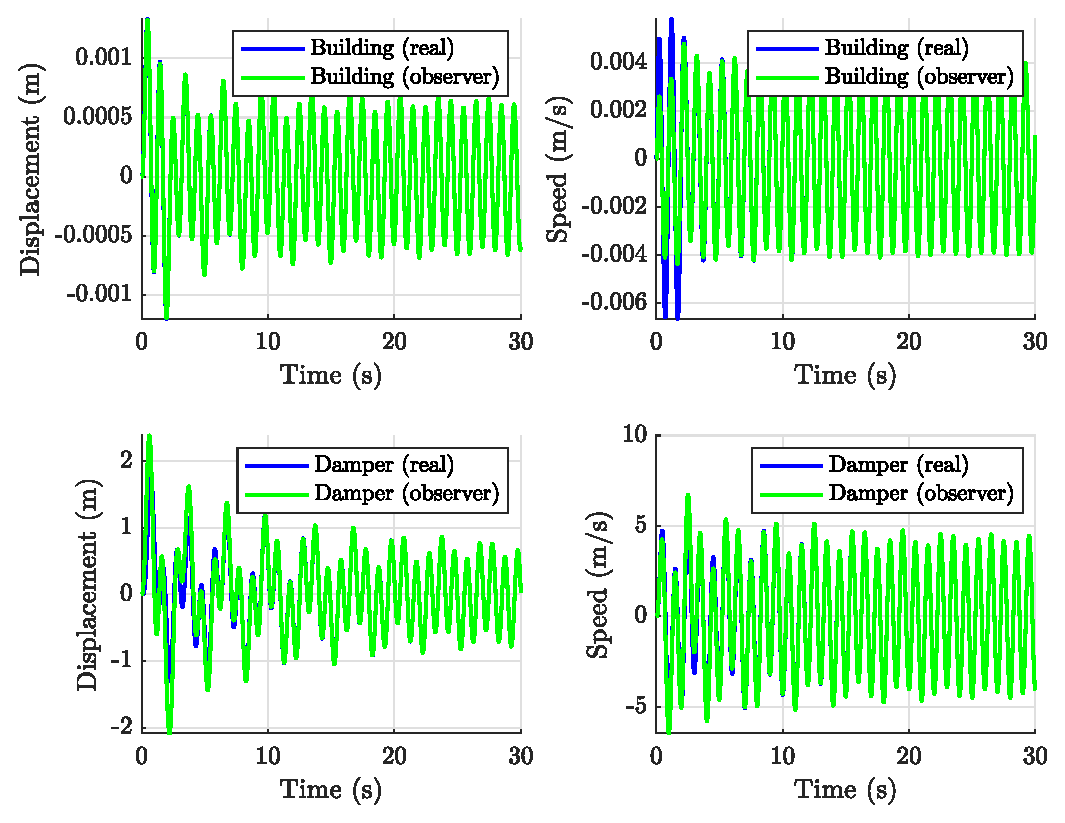
\includegraphics[width=\textwidth]{resources/eps/observer-sinusoidal.eps}
    \caption{System and observer simulation with a sinusoidal wind force}
\end{figure}
\begin{figure}[H]
    \centering
    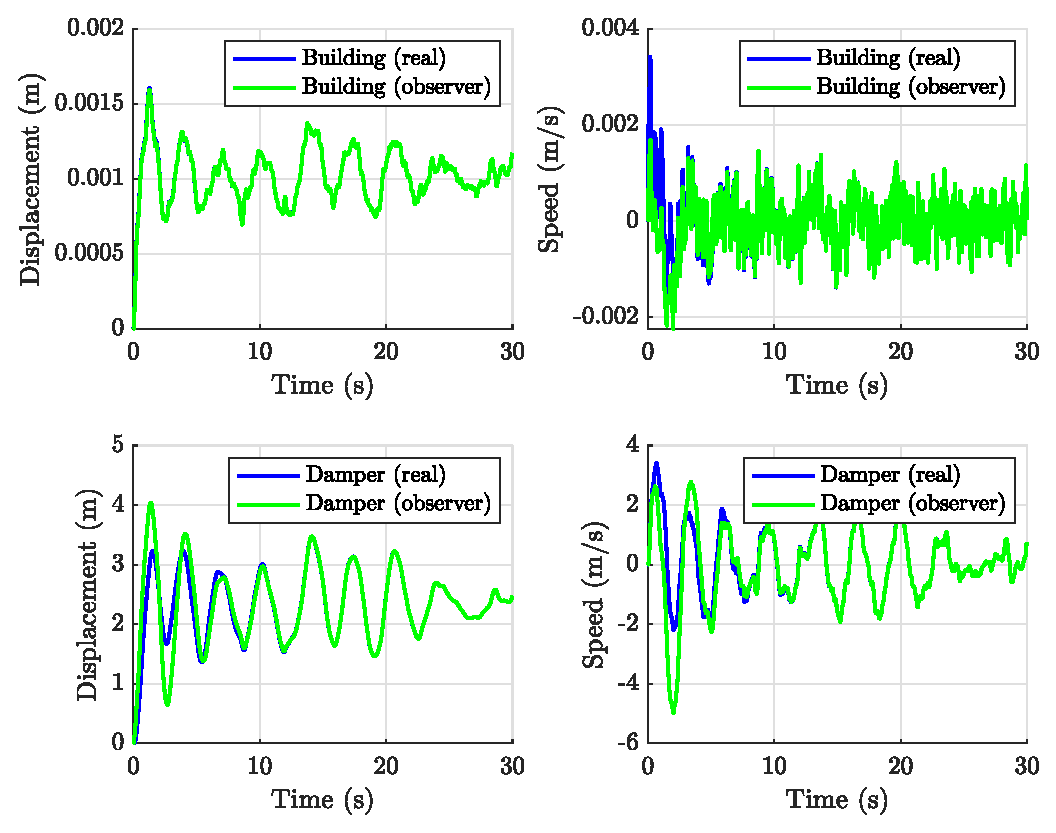
\includegraphics[width=\textwidth]{resources/eps/observer-random.eps}
    \caption{System and observer simulation with a random wind force}
\end{figure}
comments to do

\subsubsection{Presence of noise}
For this simulation, we added a random noise to the input to the observer. This one does not receive the real output of the system, but a noisy output.
\begin{figure}[H]
    \centering
    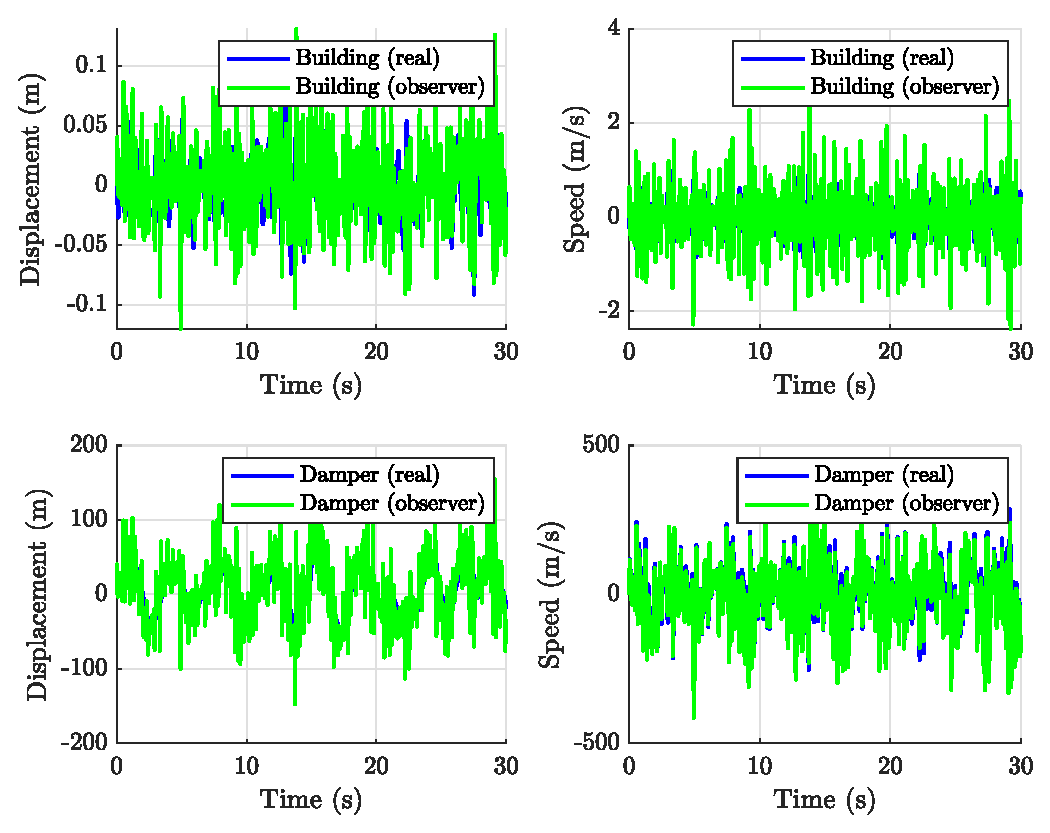
\includegraphics[width=\textwidth]{resources/eps/observer-noise.eps}
    \caption{System and observer simulation with noise in the observer}
\end{figure}
comments to do
